\section{Usecase diagram}
\subsection{Toàn bộ hệ thống}
\begin{figure}[H]
    \centering
    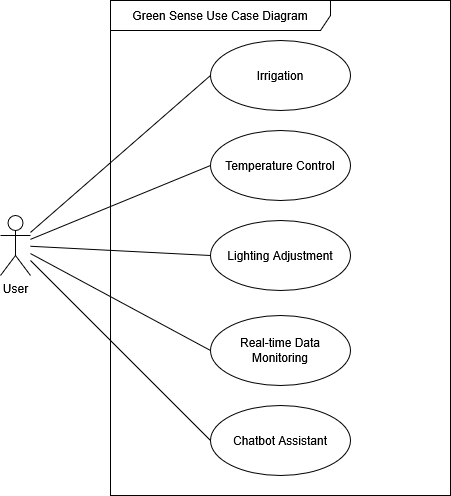
\includegraphics[width=0.85\linewidth]{content/images/GreenSense_UC_Diagram.png}
    \caption{Biểu đồ use case cho hệ thống Green Sense}
    \label{fig:useCaseDiagram}
\end{figure}
\subsection{Bảng mô tả cho từng use case}
\subsubsection{Use case 1 - Tưới nước}

\renewcommand{\arraystretch}{1.6}
\begin{table}[H]
\centering
\begin{tabular}{|p{0.2\linewidth}|p{0.7\linewidth}|}
\hline
\rowcolor[HTML]{EFEFEF} 
\textbf{Usecase}        & \textbf{Tưới nước} \\ \hline
Use case ID             & 1 \\ \hline
Actor                   & Người dùng của hệ thống \\ \hline
Description             & 
Hệ thống cung cấp ba chế độ tưới:
\begin{itemize}
    \item [--] Tự động: Duy trì độ ẩm đất theo mức cài đặt sẵn.
    \item [--] Lập lịch: Tưới theo lịch do người dùng đặt.
    \item [--] Thủ công: Người dùng tự bật/tắt tưới.
\end{itemize}
\\ \hline
Precondition            & Hệ thống đang hoạt động bình thường và được trang bị ít nhất một máy bơm, một cảm biến độ ẩm đất và một nguồn nước \\ \hline
Postcondition           & Dữ liệu độ ẩm đất được ghi lại theo tần suất mà kế hoạch hiện tại kiểm tra độ ẩm. Ngoài ra, hệ thống cũng lưu trữ nhật ký tất cả các lần tưới, kèm theo thông tin về sự kiện kích hoạt tưới. \\ \hline
Normal Flow             & 
Quy trình hoạt động dự kiến là người dùng ủy quyền việc tưới tiêu cho hệ thống.\newline
1. Người dùng mở trang web của hệ thống. \newline
3. Người dùng chọn "Tưới tiêu" từ danh sách tính năng trên giao diện chính. \newline
4. Người dùng chọn "Tự động" trong phần Chế độ. \newline
5. Người dùng đặt mức độ ẩm mục tiêu theo bảng giá trị khuyến nghị trên màn hình hoặc điều chỉnh bằng thanh trượt để chọn giá trị tùy chỉnh. \newline
6. Hệ thống đánh giá từng phép đo nhận được và thực hiện hành động nếu cần. Cụ thể, nếu độ ẩm thấp hơn 50\% so với mức mục tiêu, hệ thống sẽ tưới trong 5 giây. 
\\ \hline
Alternative Flow          & 
    Tại bước 4, nếu người dùng chọn tưới theo lịch: \newline
    4.1 Người dùng chọn thêm một nhiệm vụ tưới mới. \newline
    4.2 Người dùng chọn khoảng thời gian lập lịch (theo chế độ Cron hoặc chế độ Interval). Biểu mẫu tương ứng sẽ hiển thị. \newline
    4.3 Người dùng đặt thời gian tưới trong lịch trình đó và đặt thời gian bơm nước cần sử dụng. \newline
    4.4 Hệ thống tưới theo lịch trình đã đặt. Nếu hành động tự động được bật, hệ thống sẽ theo dõi độ ẩm đất mỗi khi có dữ liệu mới và có thể gửi cảnh báo qua thông báo nếu cần. \newline
    Tại bước 4, nếu người dùng chọn tưới hoàn toàn thủ công:\newline
    4.1 Người dùng chỉ định hệ thống bật bơm nước trong khoảng thời gian do người dùng tự thiết lập
    Chi tiết về giao diện ứng dụng có thể thay đổi trong quá trình phát triển.
 \\ \hline
\end{tabular}
\end{table}

\begin{table}[H]
\begin{tabular}{|p{0.2\linewidth}|p{0.7\linewidth}|}
    \hline
    Exception Flow          & 
        Tại bước 6, nếu hệ thống phát hiện sự thay đổi bất thường (hoặc không có thay đổi) trong độ ẩm đất khi đang tưới: \newline
        a. Hệ thống không phát hiện sự thay đổi độ ẩm nhanh như mong đợi hoặc không có thay đổi nào. \newline
        b. Hệ thống gửi thông báo đẩy đến ứng dụng trên điện thoại, cảnh báo về sự cố với nguồn nước (hết nước hoặc tắc nghẽn) hoặc bơm. \newline
        c. Nếu cơ chế dự phòng được kích hoạt, hệ thống thực hiện hành động mạnh hơn (bật bơm trong 20 giây). 
    \\ \hline
    \end{tabular}
\caption{Bảng mô tả cho use case Tưới nước}
\end{table}



\subsubsection{Use case 2 - Điều chỉnh nhiệt độ}
\renewcommand{\arraystretch}{1.6}
\begin{table}[H]
\centering
\begin{tabular}{|p{0.2\linewidth}|p{0.7\linewidth}|}
\hline
\rowcolor[HTML]{EFEFEF} 
\textbf{Usecase}        & \textbf{Điều chỉnh nhiệt độ} \\ \hline
Use case ID             & 2 \\ \hline
Actor                   & Người dùng của hệ thống \\ \hline
Description             & 
    Với tính năng kiểm soát nhiệt độ, hệ thống cung cấp 3 lựa chọn:
    \begin{itemize}
        \item [--] \textbf{Chế độ tự động:} Hệ thống cố gắng duy trì nhiệt độ bên trong nhà kính ở mức lý tưởng.
        \item [--] \textbf{Chế độ theo lịch:} Tuân theo lịch trình mà người dùng cài đặt, kèm theo tùy chọn dự phòng an toàn (nếu muốn) để hệ thống tự điều chỉnh khi có biến động bất thường.
        \item [--] \textbf{Chế độ thủ công:} Người dùng toàn quyền điều khiển đóng/mở các tấm che nắng (là những tấm che trên trần có khả năng cản sáng; trong mô hình này, chúng ta dùng động cơ mô phỏng việc cuốn/mở tấm che), bất cứ khi nào họ muốn.
    \end{itemize}
\\ \hline
Precondition            & 
Hệ thống đang vận hành bình thường. \newline
Hệ thống được trang bị cảm biến DHT20 để đo nhiệt độ và độ ẩm. \newline
Tùy chọn, hệ thống có lắp các tấm che nắng kết nối với bộ truyền động (Động cơ Servo SG90S) để cuộn vào hoặc mở ra. 
\\ \hline
Postcondition           & 
Nhiệt độ (đo bởi cảm biến) và trạng thái của tấm che nắng được ghi nhận vào cơ sở dữ liệu của hệ thống theo định kỳ. \newline
Mọi hành động điều chỉnh nhiệt độ (do người dùng thực hiện hoặc do hệ thống tự động) đều được ghi lại vào lịch sử.
\\ \hline
Normal Flow             & 
1. Người dùng mở trang web của hệ thống. \newline
2. Người dùng chọn “Temperature control” (Kiểm soát nhiệt độ) từ danh sách tính năng trên màn hình chính. \newline
3. Người dùng chọn “Scheduled mode” (Chế độ theo lịch). \newline
4. Người dùng chọn khung giờ mong muốn và chọn góc độ để tấm che nắng mở hoặc đóng.
\\ \hline
Alternative Flow 1        & 
3.1. Tại bước 3, nếu người dùng chọn “Automatic” (Tự động): \newline
3.1.1 Người dùng chỉ định khoảng nhiệt độ mục tiêu. \newline
3.1.2 Hệ thống bắt đầu kiểm tra mức nhiệt mỗi khi có dữ liệu mới từ cảm biến. Ví dụ, nếu nhiệt độ bên trong nhà kính thấp hơn khoảng mục tiêu từ 3 đến 5 độ C, hệ thống sẽ mở các tấm che nắng theo góc mà người dùng đã cài đặt từ trước
\\ \hline
Alternative Flow 2        & 
3.2. Tại bước 3, nếu người dùng chọn “Manual” (Thủ công): \newline
3.2.1 Người dùng chỉ định góc độ mà tấm che nắng sẽ mở và chọn "điều khiển tấm che nắng" \newline
3.2.2 Tấm che nắng sẽ được mở với góc độ mà người dùng đã cài đặt
\\ \hline
\end{tabular}
\caption{Bảng mô tả cho use case Điều chỉnh nhiệt độ}
\end{table}

\subsubsection{Use case 3 - Điều chỉnh ánh sáng}
\renewcommand{\arraystretch}{1.6}
\begin{table}[H]
\centering
\begin{tabular}{|p{0.2\linewidth}|p{0.7\linewidth}|}
\hline
\rowcolor[HTML]{EFEFEF} 
\textbf{Usecase}        & \textbf{Điều chỉnh ánh sáng} \\ \hline
Use case ID             & 3 \\ \hline
Actor                   & Người dùng của hệ thống \\ \hline
Description             & Chúng ta có thể tùy chỉnh cho phù hợp các mức độ ánh sáng phù hợp trong nhà trồng cây với 3 chế độ: tự động điều chỉnh phù hợp với điều kiện môi trường, lập lịch các khoảng thời gian trong ngày hoặc các ngày trong tuần, hoặc người dùng có thể điều chỉnh ánh sáng của đèn trực tiếp. \\ \hline
Precondition            & Hệ thống hoạt động bình thường và luôn được trang bị cảm biến ánh sáng và một mạch role gắn vào nguồn chiếu sáng của nguồn chiếu sáng. \\ \hline
Postcondition           & Hệ thống ánh sáng hoạt động đúng như cách người dùng thiết lập. Các hành động điều chỉnh mức độ sáng bởi người dùng hay hệ thống đều được lưu vào lịch sử theo dõi. \\ \hline
Normal Flow             & 
    1. Người dùng mở trang web của hệ thống. \newline
    2. Người dùng chọn ``Điều chỉnh chế độ sáng" từ danh sách các tính năng trên màn hình chính. \newline
    3. Người dùng chọn ``Lập lịch". \newline
    4. Hệ thống cung cấp một thanh trượt dựa trên phạm vi biểu thị 24h trong ngày. \newline
    5. Người dùng chọn khoảng thời gian mong muốn trong ngày để đèn hoạt động và các mức độ để đèn bật (với cường độ sáng tăng từ 1 đến 4, tắt đèn là 0). 
\\ \hline
Alternative Flow 1          & 
    3.1. Ở bước 3, nếu người dùng chọn `Tự động' trên thanh tùy chọn: \newline
    3.1.1. Người dùng chọn cụ thể mức độ sáng mục tiêu \newline
    3.1.2. Hệ thống bắt đầu kiểm tra và nhận dữ liệu về sau mỗi đơn vị thời gian. Nếu mức độ sáng không phù hợp với cấu hình không đúng với mục tiêu, hệ thống sẽ điều chỉnh đến khi nào cảm biến ánh sáng nhận được dữ liệu với mức độ sáng theo cách người dùng thiết lập  \\ \hline
Alternative Flow 2          & 
    3.2. Ở bước 3, nếu người dùng chọn `Thủ công' trên thanh tùy chọn: \newline
    3.2.1. Người dùng thiết lập độ sáng cho đèn (với cường độ sáng tăng từ 1 đến 4, tắt đèn là 0) và chọn ``Điều khiển đèn" \newline 
    3.2.2. Đèn sẽ được bật/tắt theo thiết lập của người dùng. \\ \hline
\end{tabular}
\caption{Bảng mô tả cho use case Điều chỉnh ánh sáng}
\end{table}

\subsubsection{Use case 4 - Theo dõi dữ liệu theo thời gian thực và thống kê hệ thống}
\renewcommand{\arraystretch}{1.6}
\begin{table}[H]
\centering
\begin{tabular}{|p{0.2\linewidth}|p{0.7\linewidth}|}
\hline
\rowcolor[HTML]{EFEFEF} 
\textbf{Usecase}        & \textbf{Theo dõi dữ liệu theo thời gian thực và thống kê hệ thống} \\ \hline
Use case ID             & 4 \\ \hline
Actor                   & Người dùng của hệ thống \\ \hline
Description             & Ứng dụng cho phép người dùng xem dữ liệu đã ghi dưới dạng báo cáo tổng hợp (trong một khoảng thời gian) với các tính toán tổng hợp và biểu đồ tổng quan về các bản ghi trước đó. \\ \hline
Precondition            & Trang web được kết nối với cơ sở dữ liệu và hệ thống vẫn đang ghi lại thống kê. \\ \hline
Postcondition           & Không có.  \\ \hline
Normal Flow             & 
    1. Người dùng mở trang web của hệ thống. \newline
    2. Người dùng chọn `Thống kê' từ danh sách các tính năng trên màn hình chính. \newline
    3. Hệ thống trích xuất dữ liệu hàng ngày làm chế độ báo cáo mặc định và hiển thị cho người dùng. Báo cáo bao gồm biểu đồ đường về mức ánh sáng, độ ẩm và nhiệt độ trong khoảng thời gian đó; các hành động đáng chú ý được thực hiện thủ công hoặc tự động trên hệ thống nhà kính; và trạng thái mới nhất của nhà kính (các phép đo nhận được gần nhất). \newline
    4. Người dùng có thể chọn khoảng thời gian ưa thích bằng cách chọn `Khoảng thời gian' trên thanh tùy chọn. \newline
    5. Hệ thống cung cấp lịch chi tiết để người dùng chọn ngày bắt đầu và ngày kết thúc cho báo cáo. \newline
    6. Người dùng chọn khoảng thời gian ưa thích và nhấn `Xác nhận'. \newline
    7. Hệ thống tải lại trang báo cáo với chế độ hiển thị biểu đồ phù hợp và theo dõi hành động. \newline
    8. Người dùng nhấn `Hoàn tất' để quay lại trang chính.
\\ \hline
Alternative Flow          & 
\\ \hline
Exception Flow          &  
\\ \hline
\end{tabular}
\caption{Bảng mô tả cho use case Theo dõi dữ liệu theo thời gian thực và thống kê hệ thống}
\end{table}

\subsubsection{Use case 5 - Điều khiển IoT Device trong hệ thống bằng Chatbox AI}

\renewcommand{\arraystretch}{1.6}
\begin{table}[H]
\centering
\begin{tabular}{|p{0.2\linewidth}|p{0.7\linewidth}|}
\hline
\rowcolor[HTML]{EFEFEF} 
\textbf{Usecase}        & \textbf{Điều khiển IoT Device trong hệ thống bằng Chatbox AI} \\ \hline
Use case ID             & 5 \\ \hline
Actor                   & Người dùng của hệ thống \\ \hline
Description             & Người dùng sử dụng khung chat trên giao diện web để gửi lệnh điều khiển thiết bị IoT bằng ngôn ngữ tự nhiên. Hệ thống AI sẽ phân tích lệnh, ánh xạ với API đã được huấn luyện và thực hiện lệnh phù hợp. \\ \hline
Precondition            & 
    - Người dùng đã đăng nhập hệ thống. \newline
    - AI được cấp quyền truy cập vào hệ thống web server. \newline
    - AI đã được huấn luyện với tài liệu API tương ứng.
\\ \hline
Postcondition           &  
    - Hệ thống thực hiện đúng lệnh điều khiển IoT nếu AI hiểu được lệnh. \newline
    - Nếu lệnh không hợp lệ hoặc không hiểu được, AI sẽ thông báo lỗi cho người dùng mà không thực hiện hành động.
\\ \hline
Normal Flow             & 
    1. Người dùng truy cập vào trang web hệ thống. \newline
    2. Người dùng chọn tính năng "Control IoT with AI helper" từ thanh công cụ. \newline
    3. Giao diện chat được hiển thị. \newline
    4. Người dùng nhập lệnh điều khiển bằng ngôn ngữ tự nhiên. \newline
    5. AI phân tích ngữ nghĩa lệnh và ánh xạ với lời gọi API phù hợp. \newline
    6. AI gửi lời gọi API đến server điều khiển IoT Device. \newline
    7. Thiết bị IoT phản hồi và thực hiện hành động.
\\ \hline
Alternative Flow          & 
\\ \hline
Exception Flow          &  
- Tại bước 5, nếu AI không hiểu lệnh (do chưa được huấn luyện hoặc lệnh không rõ ràng): \newline
+ AI thông báo lỗi: “Tôi chưa hiểu rõ lệnh này. Bạn có thể diễn đạt lại?” \newline
+ Không thực hiện gọi API.
\\ \hline
\end{tabular}
\caption{Bảng mô tả cho use case Điều khiển IoT Device trong hệ thống bằng Chatbox AI}
\end{table}

% TBU
% \renewcommand{\arraystretch}{1.6}
% \begin{table}[H]
% \centering
% \begin{tabular}{|p{0.2\linewidth}|p{0.7\linewidth}|}
% \hline
% \rowcolor[HTML]{EFEFEF} 
% \textbf{Usecase}        & \textbf{Tưới nước} \\ \hline
% Use case ID             & 5 \\ \hline
% Actor                   & Người dùng của hệ thống \\ \hline
% Description             & Lorem ipsum dolor sit amet, consectetur adipiscing elit. Nulla ut augue in odio ultricies vehicula vel quis ex. Nullam ut lacinia ex, eget maximus ante. Donec dictum rutrum efficitur. Aliquam ut dui in nunc tincidunt posuere eget vitae arcu. In eget leo id turpis scelerisque malesuada. Nam semper fringilla lorem nec ornare. Mauris gravida pharetra enim, at fermentum nunc. \\ \hline
% Precondition            & Sed laoreet ultrices lobortis. Proin pretium aliquet neque vel suscipit. Nam nec auctor sem. Orci varius natoque penatibus et magnis dis parturient montes, nascetur ridiculus mus. Maecenas tincidunt at erat porta lobortis. Aenean a tincidunt erat. Integer tempus orci a ornare feugiat. Cras eros ligula, laoreet et ante eu, consectetur lacinia mi. Cras ac porttitor ex, id facilisis tortor. Duis sit amet auctor enim. \\ \hline
% Postcondition           & Vivamus luctus lacinia ullamcorper. Fusce a fermentum nunc. Quisque luctus lobortis dolor id blandit. Donec quis tortor volutpat, vehicula lectus ac, dictum magna. Sed in sem non nisi finibus finibus. Etiam sagittis nisl sit amet urna ultrices condimentum. Donec nec molestie ligula. Vestibulum pellentesque feugiat lacus vel gravida. Vivamus sed egestas nisl. Praesent lacus  Fusce viverra purus quis eleifend gravida.  \\ \hline
% Trigger                 & Vivamus luctus lacinia ullamcorper. Fusce a fermentum nunc. Quisque luctus lobortis dolor id blandit. Donec quis tortor volutpat, vehicula lectus ac, dictum magna. Sed in sem non nisi finibus finibus. Etiam sagittis nisl sit amet urna ultrices condimentum. Donec nec molestie ligula. Vestibulum pellentesque feugiat lacus vel gravida. Vivamus sed egestas nisl. Praesent lacus  Fusce viverra purus quis eleifend gravida.  \\ \hline
% Normal Flow             & Vivamus luctus lacinia ullamcorper. Fusce a fermentum nunc. Quisque luctus lobortis dolor id blandit. Donec quis tortor volutpat, vehicula lectus ac, dictum magna. Sed in sem non nisi finibus finibus. Etiam sagittis nisl sit amet urna ultrices condimentum. Donec nec molestie ligula. Vestibulum pellentesque feugiat lacus vel gravida. Vivamus sed egestas nisl. Praesent lacus  Fusce viverra purus quis eleifend gravida.  \\ \hline
% Exception Flow          & Vivamus luctus lacinia ullamcorper. Fusce a fermentum nunc. Quisque luctus lobortis dolor id blandit. Donec quis tortor volutpat, vehicula lectus ac, dictum magna. Sed in sem non nisi finibus finibus. Etiam sagittis nisl sit amet urna ultrices condimentum. Donec nec molestie ligula. Vestibulum pellentesque feugiat lacus vel gravida. Vivamus sed egestas nisl. Praesent lacus  Fusce viverra purus quis eleifend gravida.  \\ \hline
% \end{tabular}
% \caption{Usecase specification ABC}
% \end{table}


\newpage

% Table template %

% \renewcommand{\arraystretch}{1.6}
% \begin{table}[H]
% \centering
% \begin{tabular}{|l|l|}
% \hline
% \rowcolor[HTML]{EFEFEF} 
% \textbf{Usecase}          & \textbf{Usecase ABC} \\ \hline
% Actor            & Người dùng của hệ thống \\ \hline
% Description      & \begin{tabular}[c]{@{}l@{}}Mô tả chi tiết chức năng chính  \\ Mô tả chi tiết chức năng chính\end{tabular} \\ \hline
% Precondition     & \\ \hline
% Postcondition    & \\ \hline
% Trigger          & \\ \hline
% Normal Flow      & \\ \hline
% Exception Flow   & \\ \hline
% \end{tabular}
% \caption{Usecase specification ABC}
% \end{table}